\section{Method}
\label{sec:method}

\subsection{Task, Normalization, and Patches}
Given history $X\in\mathbb R^{B\times L\times C}$, the model predicts
$\widehat Q\in\mathbb R^{B\times H\times C\times7}$ at levels
$\mathcal T=\{.05,.10,.25,.50,.75,.90,.95\}$.
A per-variable global scaler is fitted only on training observations. Model-side non-affine RevIN~\cite{kim2022revin} then normalizes each observed window:
\begin{equation}
 \widetilde X_{btc}=(X_{btc}-\mu_{bc})/s_{bc},\qquad
 s_{bc}=\sqrt{\operatorname{Var}_t(X_{btc})+10^{-5}}.
\end{equation}
Window statistics are detached from the gradient graph and use no future targets.

Length-$P$ patches at stride $S$ yield
$N=\lfloor(L-P)/S\rfloor+1$ historical tokens. An affine $P\rightarrow D$ projection and learned position embeddings form $T\in\mathbb R^{BC\times N\times D}$. Batch and variable axes are flattened, so variables share weights but do not exchange observations. With $L=336$, $P=16$, and $S=8$, $N=41$; the working width is $D=64$.

\subsection{Lightweight Historical Encoder}
Each residual token-wise MLP block computes
\begin{equation}
 T'=T+\operatorname{Drop}\!\left(W_2
 \operatorname{Drop}(\operatorname{GELU}(W_1\operatorname{LN}(T)))\right).
\end{equation}
The feature widths are $64\rightarrow128\rightarrow64$, followed after the block stack by a final layer normalization. These blocks mix features within each patch, not patch positions. Cross-patch information enters through historical pooling, decoder retrieval, and the direct correction branch.

The final configuration uses two blocks. This design retains a lightweight feature extractor while assigning history-wide retrieval to the decoder and the direct correction branch. Figure~\ref{fig:architecture} summarizes the forecasting path and its main components. Variables share model weights and are processed independently; the sampling illustrations are schematic rather than measured attention.

\begin{figure*}[t]
\centering
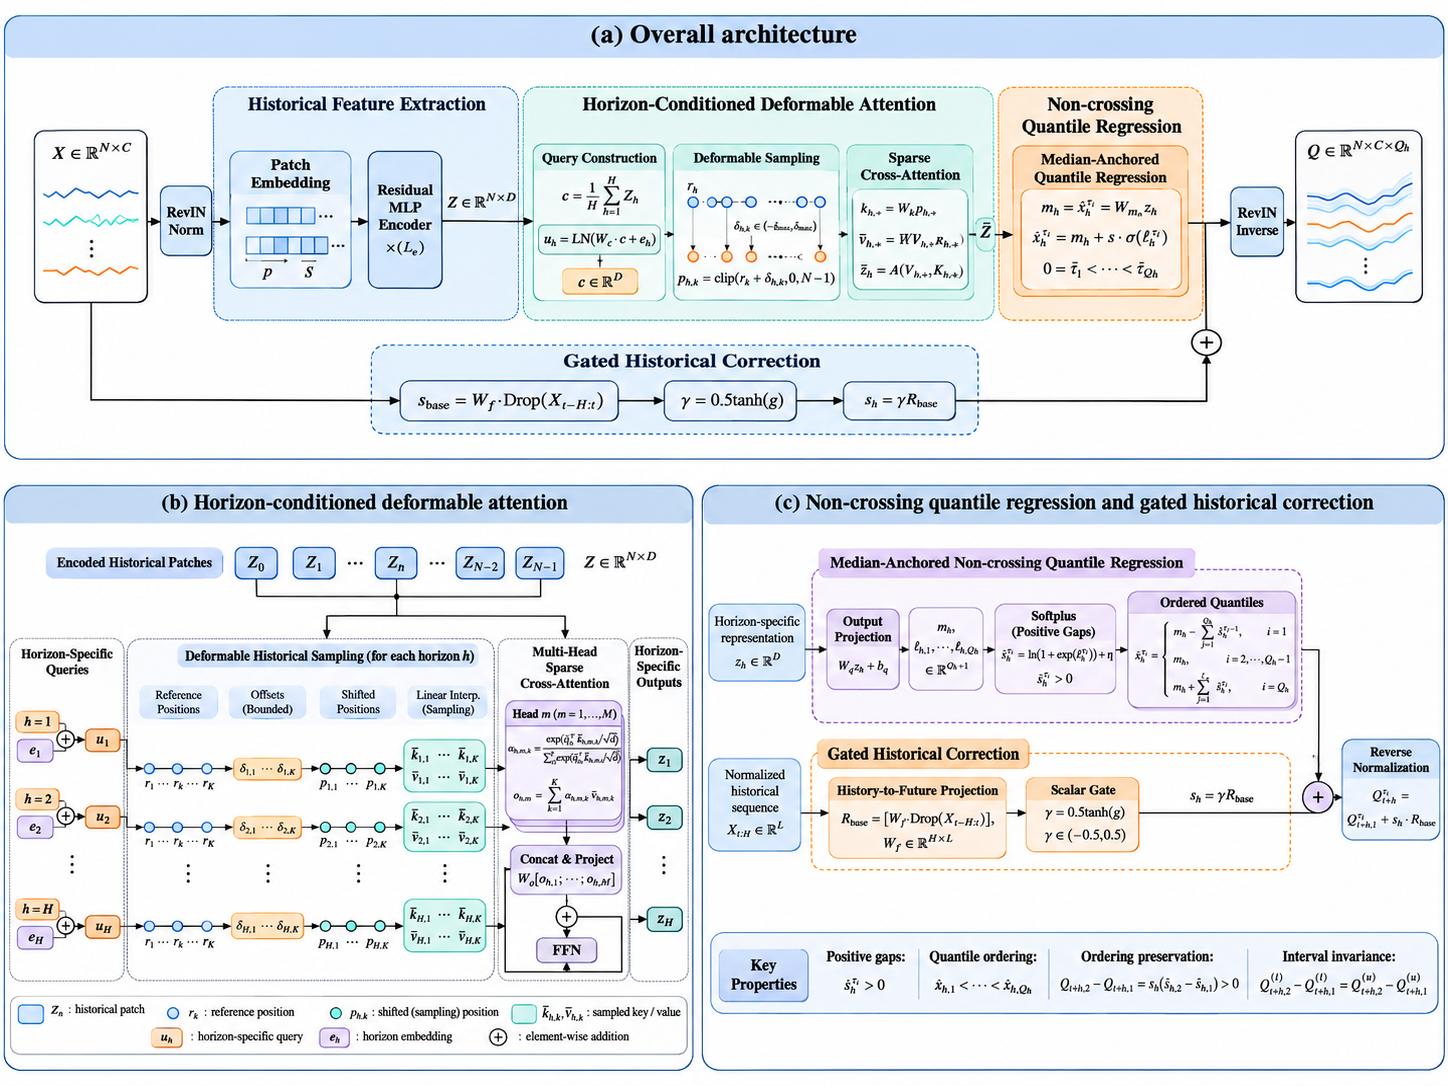
\includegraphics[width=.98\textwidth]{figures/architecture_draft.png}
\caption{Overall architecture of HDA-NQ.}
\Description{A forecasting path and an expanded decoder show normalization, patches, residual MLP encoding, future-step queries, sparse interpolation, attention, ordered quantiles, and a common history correction.}
\label{fig:architecture}
\end{figure*}

\subsection{Horizon-Conditioned Deformable Retrieval}
Suppressing batch and variable indices, let $Z\in\mathbb R^{N\times D}$ be encoded history. Future step $h$ receives a learned embedding $e_h$ and a history-conditioned query base:
\begin{equation}
 u_h=\operatorname{LN}\!\left(W_c\,N^{-1}\sum_nZ_n+e_h\right).
 \label{eq:query}
\end{equation}
For head $m$ and sample $k$, predicted offsets adjust uniform reference positions:
\begin{equation}
 \begin{aligned}
 r_k&=(k-1)(N-1)/(K-1),\\
 \delta_{hmk}&=a\tanh([W_\delta u_h]_{mk}),\\
 p_{hmk}&=\operatorname{clip}(r_k+\delta_{hmk},0,N-1).
 \end{aligned}
 \label{eq:offset}
\end{equation}
The configuration uses $M=8$ heads, $K=8$ samples, and $a=1.5$ patch tokens. Offset projections start at zero. The grid spans the whole history, but each sample moves only within a bounded neighborhood; sampling is not unrestricted global relocation. Clipping can hold endpoint samples at the boundary. In particular, the interpolation neighbors coincide at the rightmost reference; its zero-initialized offset receives no interpolation gradient and retains the most recent patch as an endpoint anchor.

Queries, keys, and values are affine projections of $u_h$ and $Z$, split into heads of width $d=D/M$. For either projected history $F$, a continuous location $p$ is sampled by
\begin{equation}
 \mathcal I(F,p)=(1-\lambda)F_\ell+\lambda F_r,\quad
 \ell=\lfloor p\rfloor,\ r=\min(\ell+1,N-1),\
 \lambda=p-\ell.
\end{equation}
Only neighboring features are gathered. Attention is normalized over the sampled locations within each head:
\begin{align}
 \alpha_{hmk}&=\operatorname{softmax}_k
 \left(q_{hm}^{\mathsf T}\mathcal I(K_m,p_{hmk})/\sqrt d\right),\\
 o_{hm}&=\sum_k\alpha_{hmk}\mathcal I(V_m,p_{hmk}).
\end{align}
The combined heads undergo residual refinement:
\begin{align}
 v_h&=\operatorname{LN}_1\!\left(u_h+\operatorname{Drop}(W_O[o_{h1};\ldots;o_{hM}])\right),\\
 z_h&=v_h+\operatorname{Drop}(\operatorname{FFN}(\operatorname{LN}_2(v_h))).
\end{align}
The decoder FFN has widths $D\rightarrow2D\rightarrow D$. Queries do not access future targets or attend to other future queries. Horizon chunking changes memory use without changing these dependencies.

\subsection{Ordered Outputs and Common Correction}
An affine projection of $z_h$ produces median $m_h$ and six gap logits. Positive gaps
$g^\pm_{hj}=\operatorname{softplus}(a^\pm_{hj})+\eta$,
$j=1,2,3$, $\eta=10^{-4}$, define
\begin{equation}
 \widetilde q_{h,4}=m_h,\qquad
 \widetilde q_{h,4\pm j}=m_h\pm\sum_{i=1}^jg^\pm_{hi}.
 \label{eq:ordering}
\end{equation}
Indices follow ascending quantile levels; negative-side cumulative outputs are reversed into ascending order. Reverse RevIN returns
$Q^{base}_{bhcq}=s_{bc}\widetilde q_{bhcq}+\mu_{bc}$.

A direct history correction is added to the base output:
\begin{equation}
 \begin{aligned}
 R_{bhc}&=[W_R\operatorname{Drop}(\widetilde X_{b,:,c})]_h,\\
 \gamma&=0.5\tanh(g),\\
 \widehat Q_{bhcq}&=Q^{base}_{bhcq}+s_{bc}\gamma R_{bhc}.
 \end{aligned}
 \label{eq:correction}
\end{equation}
Here $W_R\in\mathbb R^{H\times L}$ has no bias and starts at zero; the gate starts at $\gamma=0.1$. The bounded gate does not bound correction amplitude because $W_R$ is trainable. The same correction shifts every quantile, supplying a direct history-to-future path without changing interval widths for fixed base outputs.

\noindent\textbf{Ordering property.}
Adjacent cumulative outputs in Eq.~\eqref{eq:ordering} differ by a positive gap. Multiplication by $s_{bc}>0$, addition of $\mu_{bc}$, and the common shift in Eq.~\eqref{eq:correction} preserve their order. In floating-point computation, rounding may produce ties. Ordering establishes neither nominal coverage nor simultaneous uncertainty across variables and future steps.

\subsection{Objective and Computational Scope}
All working configurations minimize mean pinball loss:
\begin{equation}
 \begin{aligned}
 \mathcal L&=\frac{1}{7BHC}\sum_{b,h,c,q}
 \max\{\tau_q e_{bhcq},(\tau_q-1)e_{bhcq}\},\\
 e_{bhcq}&=Y_{bhc}-\widehat Q_{bhcq}.
 \end{aligned}
\end{equation}
No difference auxiliary loss or post-hoc calibration is used. With $K<N$, sampled attention scores and aggregation cost $O(BCHKD)$ rather than $O(BCHND)$ for dense historical attention. This comparison excludes projections, FFNs, the encoder, and the $O(BCLH)$ history correction. It therefore does not imply lower end-to-end latency; no hardware speedup claim is made.
